%% This file was auto-generated by IPython.
%% Conversion from the original notebook file:
%% svdrecom.ipynb
%%
\documentclass[11pt,english,fleqn]{article}

%% This is the automatic preamble used by IPython.  Note that it does *not*
%% include a documentclass declaration, that is added at runtime to the overall
%% document.

\usepackage{amsmath}
\usepackage{amssymb}
\usepackage{graphicx}
\usepackage{ucs}
\usepackage[utf8x]{inputenc}

% needed for markdown enumerations to work
\usepackage{enumerate}

% Slightly bigger margins than the latex defaults
\usepackage{geometry}
\geometry{verbose,tmargin=3cm,bmargin=3cm,lmargin=2.5cm,rmargin=2.5cm}

% Define a few colors for use in code, links and cell shading
\usepackage{color}
\definecolor{orange}{cmyk}{0,0.4,0.8,0.2}
\definecolor{darkorange}{rgb}{.71,0.21,0.01}
\definecolor{darkgreen}{rgb}{.12,.54,.11}
\definecolor{myteal}{rgb}{.26, .44, .56}
\definecolor{gray}{gray}{0.45}
\definecolor{lightgray}{gray}{.95}
\definecolor{mediumgray}{gray}{.8}
\definecolor{inputbackground}{rgb}{.95, .95, .85}
\definecolor{outputbackground}{rgb}{.95, .95, .95}
\definecolor{traceback}{rgb}{1, .95, .95}

% Framed environments for code cells (inputs, outputs, errors, ...).  The
% various uses of \unskip (or not) at the end were fine-tuned by hand, so don't
% randomly change them unless you're sure of the effect it will have.
\usepackage{framed}

% remove extraneous vertical space in boxes
\setlength\fboxsep{0pt}

% codecell is the whole input+output set of blocks that a Code cell can
% generate.

% TODO: unfortunately, it seems that using a framed codecell environment breaks
% the ability of the frames inside of it to be broken across pages.  This
% causes at least the problem of having lots of empty space at the bottom of
% pages as new frames are moved to the next page, and if a single frame is too
% long to fit on a page, will completely stop latex from compiling the
% document.  So unless we figure out a solution to this, we'll have to instead
% leave the codecell env. as empty.  I'm keeping the original codecell
% definition here (a thin vertical bar) for reference, in case we find a
% solution to the page break issue.

%% \newenvironment{codecell}{%
%%     \def\FrameCommand{\color{mediumgray} \vrule width 1pt \hspace{5pt}}%
%%    \MakeFramed{\vspace{-0.5em}}}
%%  {\unskip\endMakeFramed}

% For now, make this a no-op...
\newenvironment{codecell}{}

 \newenvironment{codeinput}{%
   \def\FrameCommand{\colorbox{inputbackground}}%
   \MakeFramed{\advance\hsize-\width \FrameRestore}}
 {\unskip\endMakeFramed}

\newenvironment{codeoutput}{%
   \def\FrameCommand{\colorbox{outputbackground}}%
   \vspace{-1.4em}
   \MakeFramed{\advance\hsize-\width \FrameRestore}}
 {\unskip\medskip\endMakeFramed}

\newenvironment{traceback}{%
   \def\FrameCommand{\colorbox{traceback}}%
   \MakeFramed{\advance\hsize-\width \FrameRestore}}
 {\endMakeFramed}

% Use and configure listings package for nicely formatted code
\usepackage{listingsutf8}
\lstset{
  language=python,
  inputencoding=utf8x,
  extendedchars=\true,
  aboveskip=\smallskipamount,
  belowskip=\smallskipamount,
  xleftmargin=2mm,
  breaklines=true,
  basicstyle=\small \ttfamily,
  showstringspaces=false,
  keywordstyle=\color{blue}\bfseries,
  commentstyle=\color{myteal},
  stringstyle=\color{darkgreen},
  identifierstyle=\color{darkorange},
  columns=fullflexible,  % tighter character kerning, like verb
}

% The hyperref package gives us a pdf with properly built
% internal navigation ('pdf bookmarks' for the table of contents,
% internal cross-reference links, web links for URLs, etc.)
\usepackage{hyperref}
\hypersetup{
  breaklinks=true,  % so long urls are correctly broken across lines
  colorlinks=true,
  urlcolor=blue,
  linkcolor=darkorange,
  citecolor=darkgreen,
  }

% hardcode size of all verbatim environments to be a bit smaller
\makeatletter 
\g@addto@macro\@verbatim\small\topsep=0.5em\partopsep=0pt
\makeatother 

% Prevent overflowing lines due to urls and other hard-to-break entities.
\sloppy

\setlength{\mathindent}{0pt}
\setlength{\parindent}{0pt}
\setlength{\parskip}{8pt}
\begin{document}

SVD, Toplu Tavsiye (Collaborative Filtering)

Diyelim ki Star Trek (ST) dizisini ne kadar begendigini 4 tane kullanici
sezonlara gore isaretlemis. Bu ornek veriyi alttaki gibi gosterelim.

\begin{codecell}
\begin{codeinput}
\begin{lstlisting}
from pandas import *

d =  np.array(
     [[5, 5, 0, 5],
     [5, 0, 3, 4],
     [3, 4, 0, 3],
     [0, 0, 5, 3],
     [5, 4, 4, 5],
     [5, 4, 5, 5]])

data = DataFrame (d.T,
    columns=['S1','S2','S3','S4','S5','S6'],
    index=['Ben','Tom','John','Fred']
    )
data
\end{lstlisting}
\end{codeinput}
\begin{codeoutput}
\begin{verbatim}
      S1  S2  S3  S4  S5  S6
Ben    5   5   3   0   5   5
Tom    5   0   4   0   4   4
John   0   3   0   5   4   5
Fred   5   4   3   3   5   5
\end{verbatim}
\end{codeoutput}
\end{codecell}
Veriye gore Tom, ST dizisinin 3. sezonunu 4 seviyesinde sevmis. 0 degeri
o sezonun seyredilmedigini gosteriyor.

Toplu Tavsiye algoritmalari verideki diger kisilerin bir urunu, diziyi,
vs.~ne kadar begendiginin verisinin diger ``benzer'' kisilere tavsiye
olarak sunabilir, ya da ondan once, bir kisinin daha almadigi urunu,
seyretmedigi sezonu, dinlemedigi muzigi ne kadar ``begeneceginin''
tahmin eder. Kaggle sitesi uzerinden yapilan unlu Netflix yarismasinin
amaci buydu - ayrica tahmin edilen ve gercek begeni notunun hata payinin
hesabi icin RMSE hesabi kullanilmisti.

Peki benzerligin kriteri nedir, ve benzerlik nelerin arasinda olculur?

Benzerlik, urun seviyesinde, ya da kisi seviyesinde yapilabilir. Eger
urun sevisinde ise, tek bir urun icin tum kullanicilarin verdigi nota
bakilir. Eger kullanici seviyesinde ise, tek kullanicinin tum urunlere
verdigi begeni notlari vektoru kullanilir.

Mesela 1. sezondan hareketle, o sezonu begenen kisilere o sezona benzer
diger sezonlar tavsiye edilebilir. Kisiden hareketle, mesela John'a
benzeyen diger kisiler bulunarak onlarin begendigi urunler John'a
tavsiye edilebilir.

Urun ya da kisi bazinda olsun, benzerligi hesaplamanin da farkli yollari
var. Genel olarak benzerlik olcutunun 0 ile 1 arasinda degisen bir sayi
olmasini tercih ediyoruz ve tum ayarlari ona gore yapiyoruz. Diyelim ki
ki elimizde begeni notlarini tasiyan $A,B$ vektorleri var (baska veri
turu de tasiyor olabilir tabii), ve bu vektorlerin icinde begeni notlari
var. Benzerlik cesitleri soyle:

Oklit Benzerligi (Euclidian Similarity)

Bu benzerlik $1 / (1+mesafe)$ olarak hesaplanir. Mesafe karelerin
toplaminin karekoku (yani Oklitsel mesafe, ki isim buradan geliyor). Bu
yuzden mesafe 0 ise (yani iki ``sey'' arasinda hic mesafe yok,
birbirlerine cok yakinlar), o zaman hesap 1 dondurur (mukemmel
benzerlik). Mesafe arttikca bolen buyudugu icin benzerlik sifira
yaklasir.

Pearson Benzerligi

Bu benzerligin Oklit'ten farkliligi, sayi buyuklugune hassas
olmamasidir. Diyelim ki birisi her sezonu 1 ile begenmis, digeri 5 ile
begenmis, bu iki vektorun Pearson benzerligine gore birbirine esit
cikar. Pearson -1 ile +1 arasinda bir deger dondurur, alttaki hesap onu
normalize ederek 0 ile 1 arasina ceker.

Kosinus Benzerligi (Cosine Similarity)

Iki vektoru geometrik vektor olarak gorur ve bu vektorlerin arasinda
olusan aciyi (daha dogrusu onun kosinusunu) farklilik olcutu olarak
kullanir.
\[
\cos\theta = \frac{A \cdot B}{||A||||B||}
\]
\begin{codecell}
\begin{codeinput}
\begin{lstlisting}
from numpy import linalg as la
def euclid(inA,inB):
    return 1.0/(1.0 + la.norm(inA - inB))

def pearson(inA,inB):
    if len(inA) < 3 : return 1.0
    return 0.5+0.5*np.corrcoef(inA, inB, rowvar = 0)[0][1]

def cos_sim(inA,inB):
    num = float(np.dot(inA.T,inB))
    denom = la.norm(inA)*la.norm(inB)
    return 0.5+0.5*(num/denom)

\end{lstlisting}
\end{codeinput}
\begin{codeoutput}
\begin{verbatim}

\end{verbatim}
\end{codeoutput}
\end{codecell}
\begin{codecell}
\begin{codeinput}
\begin{lstlisting}
print np.array(data.ix['Fred'])
print np.array(data.ix['John'])
print np.array(data.ix['Ben'])
print pearson(data.ix['Fred'],data.ix['John'])
print pearson(data.ix['Fred'],data.ix['Ben'])

\end{lstlisting}
\end{codeinput}
\begin{codeoutput}
\begin{verbatim}
[5 4 3 3 5 5]
[0 3 0 5 4 5]
[5 5 3 0 5 5]
0.551221949943
0.906922851283
\end{verbatim}
\end{codeoutput}
\end{codecell}
\begin{codecell}
\begin{codeinput}
\begin{lstlisting}
print cos_sim(data.ix['Fred'],data.ix['John'])
print cos_sim(data.ix['Fred'],data.ix['Ben'])

\end{lstlisting}
\end{codeinput}
\begin{codeoutput}
\begin{verbatim}
0.898160909799
0.977064220183
\end{verbatim}
\end{codeoutput}
\end{codecell}
Simdi tavsiye mekanigine gelelim. En basit tavsiye yontemi, mesela kisi
bazli olarak, bir kisiye en yakin diger kisileri bulmak (matrisin
tamamina bakarak) ve onlarin begendikleri urunu istenilen kisiye tavsiye
etmek. Benzerlik icin ustteki olcutlerden birini kullanmak.

Fakat belki de elimizde cok fazla urun, ya da kullanici var. Bir boyut
azaltma islemi yapamaz miyiz?

Evet. SVD yontemi burada da isimize yarar.
\[ A = USV  \]
elde edecegimiz icin, ve $S$ icindeki en buyuk degerlere tekabul eden
$U,V$ degerleri siralanmis olarak geldigi icin $U,V$'nin en bastaki
degerlerini almak bize ``en onemli'' bloklari verir. Bu en onemli kolon
ya da satirlari alarak azaltilmis bir boyut icinde benzerlik hesabi
yapmak islemlerimizi hizlandirir. Bu azaltilmis boyutta kumeleme
algoritmalarini devreye sokabiliriz; $U$'nun mesela en onemli iki kolonu
bize iki boyuttaki sezon kumelerini verebilir, $V$'nin en onemli iki (en
ust) satiri bize iki boyutta bir kisi kumesi verebilir.

O zaman begeni matrisi uzerinde SVD uygulayalim,

\begin{codecell}
\begin{codeinput}
\begin{lstlisting}
from numpy.linalg import linalg as la
U,Sigma,V=la.svd(data, full_matrices=False)
print data.shape
print U.shape, Sigma.shape, V.shape
u = U[:,:2]
vt=V[:2,:].T
print 'u', u
print 'vt', vt
print u.shape, vt.shape
\end{lstlisting}
\end{codeinput}
\begin{codeoutput}
\begin{verbatim}
(4, 6)
(4, 4) (4,) (4, 6)
u [[-0.57098887 -0.22279713]
 [-0.4274751  -0.51723555]
 [-0.38459931  0.82462029]
 [-0.58593526  0.05319973]]
vt [[-0.44721867 -0.53728743]
 [-0.35861531  0.24605053]
 [-0.29246336 -0.40329582]
 [-0.20779151  0.67004393]
 [-0.50993331  0.05969518]
 [-0.53164501  0.18870999]]
(4, 2) (6, 2)
\end{verbatim}
\end{codeoutput}
\end{codecell}
degerleri elimize gecer. U ve VT matrisleri

\begin{codecell}
\begin{codeinput}
\begin{lstlisting}
def label_points(d,xx,yy,style):
    for label, x, y in zip(d, xx, yy):
        plt.annotate(
            label, 
            xy = (x, y), xytext = style,
            textcoords = 'offset points', ha = 'right', va = 'bottom',
            bbox = dict(boxstyle = 'round,pad=0.5', fc = 'yellow', alpha = 0.5),
            arrowprops = dict(arrowstyle = '->', connectionstyle = 'arc3,rad=0'))

plot(u[:,0],u[:,1],'r.')
label_points(data.index, u[:, 0], u[:, 1],style=(-10, 30))
plot(v.T[:,0],v.T[:,1],'b.')
label_points(data.columns, vt[:, 0], vt[:, 1],style=(20, 20))


\end{lstlisting}
\end{codeinput}
\begin{codeoutput}
\begin{center}
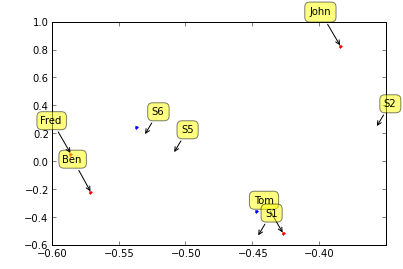
\includegraphics[width=0.7\textwidth]{svdrecom_files/svdrecom_fig_00.png}
\par
\end{center}
\end{codeoutput}
\end{codecell}
Cok guzel! SVD bize urun bazinda sezon 5 ve 6'nin bir kume
olusturdugunu, Ben ve Fred'in de kisi bazinda ayri bir kume oldugunu
gosterdi.

Azaltilmis boyutlari nasil kullaniriz? Yeni bir kisiyi (mesela Bob) ele
alinca, bu kisinin verisini oncelikle aynen diger verilerin indirgendigi
gibi azaltilmis boyuta ``indirgememiz'' gerekiyor. Cunku artik islem
yaptigimiz boyut orasi. Peki bu indirgemeyi nasil yapariz? SVD genel
formulunu hatirlarsak,
\[ A = USV \]
Azaltilmis ortamda
\[ A = U_k S_k V_k \]
Diyelim ki gitmek istedigimiz nokta azaltilmis $U$, o zaman $U_k$'yi tek
basina birakalim,
\[ A V_k^{-1} = U_k S V_k V_k^{-1} \]
$U_k,V_k$ matrisleri ortonormal, o zaman $V_k^{-1}V_k = I$ olacak, yani
yokolacak
\[ A V_k^{-1} = U_k S  \]
Benzer sekilde
\[  A V_k^{-1} S^{-1} = U_k \]
Cok fazla ters alma islemi var, her iki tarafin devrigini alalim
\[ (S^{-1})^T (V_k^{-1})^T A^T = U_k^T \]
$V_k^{-1} = V_k^T$ o zaman ustteki formul devrigin devrigini almak
demektir, yani tekrar basa donmus oluyoruz, demek ki $V_k$ degismeden
kaliyor
\[ (S^{-1})^T V_k A^T = U_k^T \]
$S$ ise kosegen matris, onun tersi yine kosegen, kosegen matrisin
devrigi yine kendisi
\[ S^{-1} V_k A^T = U_k^T \]
Bazi kod ispatlari, $u$'nun ortonormal olmasi:

\begin{codecell}
\begin{codeinput}
\begin{lstlisting}
np.dot(u.T,u)
\end{lstlisting}
\end{codeinput}
\begin{codeoutput}
\begin{verbatim}
array([[  1.00000000e+00,   4.83147593e-18],
       [  4.83147593e-18,   1.00000000e+00]])
\end{verbatim}
\end{codeoutput}
\end{codecell}
Dogal olarak ..e-17 gibi bir sayi sifira cok yakin, yani sifir kabul
edilebilir. Devrik ve tersin ayni oldugunu gosterelim: Iki matrisi
birbirinden cikartip, cok kucuk bir sayidan buyukluge gore filtreleme
yapalim, ve sonuc icinde bir tane bile True olup olmadigini kontrol
edelim,

\begin{codecell}
\begin{codeinput}
\begin{lstlisting}
not any(U.T-la.inv(U) > 1e-15)
\end{lstlisting}
\end{codeinput}
\begin{codeoutput}
\begin{verbatim}
True
\end{verbatim}
\end{codeoutput}
\end{codecell}
Yeni Bob verisi

\begin{codecell}
\begin{codeinput}
\begin{lstlisting}
bob = np.array([5,5,0,0,0,5]) 
\end{lstlisting}
\end{codeinput}
\end{codecell}
O zaman

\begin{codecell}
\begin{codeinput}
\begin{lstlisting}
print bob.T.shape
print u.shape
S_k = np.eye(2)*Sigma[:2]
bob_2d = np.dot(np.dot(la.inv(S_k),vt.T),bob.T)
print bob_2d
\end{lstlisting}
\end{codeinput}
\begin{codeoutput}
\begin{verbatim}
(6,)
(4, 2)
[-0.37752201 -0.08020351]
\end{verbatim}
\end{codeoutput}
\end{codecell}
Ustte eye ve Sigma ile ufak bir takla attik, bunun sebebi svd
cagrisindan gelen Sigma sonucunun bir vektor olmasi ama ustteki islem
icin kosegen bir ``matrise'' ihtiyacimiz olmasi. Eger birim (identity)
matrisini alip onu Sigma ile carparsak, bu kosegen matrisi elde ederiz.

Simdi mesela kosinus benzerligi kullanarak bu izdusumlenmis yeni
vektorun hangi diger vektorlere benzedigini bulalim.

\begin{codecell}
\begin{codeinput}
\begin{lstlisting}
for i,user in enumerate(u):
   print data.index[i],cos_sim(user,bob_2d)
\end{lstlisting}
\end{codeinput}
\begin{codeoutput}
\begin{verbatim}
Ben 0.993397525045
Tom 0.891664622942
John 0.612561691287
Fred 0.977685793579
\end{verbatim}
\end{codeoutput}
\end{codecell}
Sonuca gore yeni kullanici Bob, en cok Ben ve Fred'e benziyor. Sonuca
eristik! Artik bu iki kullanicinin yuksek not verdigi ama Bob'un hic not
vermedigi sezonlari alip Bob'a tavsiye olarak sunabiliriz.

\subsection{Movielens 1M Verisi}

Bu veri seti 6000 kullanici tarafindan yaklasik 4000 tane filme verilen
not / derece (rating) verisini iceriyor, 1 milyon tane not verilmis,
yani 4000 * 6000 = 24 milyon olasilik icinde sadece 1 milyon veri
noktasi dolu. Bu oldukca seyrek bir matris demektir.

Verinin ham hali diger ders notlarini da iceren ust dizinlerde var,
veriyi SVD ile kullanilir hale getirmek icin movielens\_prep.py adli
script kullanilir. Islem bitince movielens.csv adli bir dosya script'te
gorulen yere yazilacak. Bu dosyada olmayan derecelendirmeler bos
olacaktir . Bu bosluklari sifirlarsak, scipy seyrek matrisi o noktalari
atlayacaktir. Ardindan bu seyrek matris uzerinde SVD isletilebilir.

Tavsiye kodlamamiz icin yazinin basinda anlatilan teknigi kullanacagiz,
film verisi uzerinde boyut azaltilmasi yapilacak, benzer kullanici
bulunacak, ve herhangi bir yeni kullanici / film kombinasyonu icin bu
diger benzer kullanicinin o filme verdigi not baz alinacak.

Veriyi egitim ve test olarak iki parcaya bolecegiz. SVD egitim bolumu
uzerinde isletilecek.

Bu baglamda, onemli bir diger konu eksik veri noktalarinin SVD
sonuclarini etkileyip etkilemeyecegi. Sonucta eksik yerler nan, oradan
sifir yapilip ardindan seyrek matris kodlamasi uzerinden ``atlaniyor''
olabilir, fakat bu degerler atlaniyor (yani hizli isleniyor,
depolaniyor) olsa bile, onlarin sifir olmasinin bir anlami yok mudur?
Evet vardir. Not bakimindan sifir da bir not'tur, ve bu sebeple
sonuclari istenmeyen bicimde etkileyebilir.

O zaman mevcut veriyi oyle bir degistirelim ki verilmemis notlar, yani
sifir degerleri sonucu fazla degistirmesin.

Bunu yapmanin yollarindan biri her film icin bir ortalama not degeri
hesaplamak, ve bu ortalama degeri o filme verilen tum not degerlerinden
cikartmaktir. Bu isleme ``sifir cevresinde merkezlemek'' ismi de
verilir, hakikaten mesela film j icin ortalama 3 ise, 5 degeri 2, 3
degeri sifir, 2 degeri -1 olacaktir.

Altta Pandas mean cagrisi ile bu islemin yapildigini goruyoruz, dikkat,
Pandas dataframe icinde nan degerleri olacaktir, ve Pandas bu degerleri
atlamasi gerektigini bilir, yani bu degerler ortalamaya etki etmez.
Ardindan merkezleme islemi egitim verisi uzerinde uygulaniyor.

\begin{codecell}
\begin{codeinput}
\begin{lstlisting}
import pandas as pd, os
import numpy as np
import scipy.sparse as sps
df = pd.read_csv("%s/Downloads/movielens.csv" % os.environ['HOME'],sep=';')
print df.shape
df = df.ix[:,1:] # id kolonunu atla
df = df.ix[:,:3700] # sadece filmleri al
df_train = df.copy().ix[:5000,:]
df_test = df.copy().ix[5001:,:]
df_train[np.isnan(df_train)] = 0.0
movie_avg_rating = np.array(df_train.mean(axis=0))
df_train = df_train - movie_avg_rating
dfs_train = sps.coo_matrix(df_train)

df_train = np.array(df_train)
df_test = np.array(df_test)

print df_train.shape
print df_test.shape

__top_k__ = 10
import scipy.sparse.linalg as slin
import scipy.linalg as la
U,Sigma,V=slin.svds(dfs_train,k=__top_k__)
print U.shape, Sigma.shape, V.shape
Sigma = np.diag(Sigma)

\end{lstlisting}
\end{codeinput}
\begin{codeoutput}
\begin{verbatim}
(6040, 3731)
(5001, 3700)
\end{verbatim}
\begin{verbatim}
(1039, 3700)
(5001, 10)
\end{verbatim}
\begin{verbatim}
(10,) (10, 3700)
\end{verbatim}
\end{codeoutput}
\end{codecell}
Altta test verisi uzerinde satir satir ilerliyoruz, ve her satir (ayni
test kullanicisi) film film ilerliyoruz, onlara teker teker bakiyoruz.
Ilk once ``verilmis bir not'' ariyoruz (cogunlukla not verilmemis oluyor
cunku), buldugumuz zaman artik elimizde test edebilecegimiz bir sey var,
o notu ``sifirlayip'' vektorun geri kalanini azaltilmis boyuta
yansitiyoruz, ve sonra o boyuttaki tum diger $U$ vektorleri icinde arama
yapiyoruz, en yakin diger kullaniciyi buluyoruz ve onun filme verdigi
notu tahminimiz olarak kullaniyoruz.

Alttaki kodda, basitlestirme amacli olarak, eger bulunan diger kullanici
o filme not vermemisse, o filmi atliyoruz. Gercek dunya sartlarinda o
filme not vermis ve hala yakin olan (en yakin olmasa da) baska bir
kullanici bulup onun notu kullanilabilir.

\begin{codecell}
\begin{codeinput}
\begin{lstlisting}
def euclid(inA,inB):
    return 1.0/(1.0 + la.norm(inA - inB))
    
rmse = 0; n = 0
for i,test_row in enumerate(df_test):
    for j, test_val in enumerate(test_row):
        if np.isnan(test_val): continue	
	curr = test_row.copy()
        curr[j] = np.nan
        curr[np.isnan(curr)] = 0.

	proj_row = np.dot(np.dot(la.inv(Sigma),V),curr)

	sims = np.array(map(lambda x: euclid(x, proj_row), U[:,:__top_k__]))
	isim = np.argmax(sims)

	# eger bulunan kullanici o filme not vermemisse atla
	if np.isnan(df.ix[isim, j]): continue

	# egitim verisinde notlar sifir etrafinda ortalanmis, tekrar
	# normal haline dondur
	est = df_train[isim, j]+movie_avg_rating[j]

	# gercek not
	real = df_test[i, j]

	print i, 'icin en yakin', isim, 'urun',j, 'icin oy', est, 'gercek', real
        rmse += (real-est)**2
        n += 1
	break
    if i == 20: break

print "rmse", np.sqrt(rmse / n)
\end{lstlisting}
\end{codeinput}
\begin{codeoutput}
\begin{verbatim}
0 icin en yakin 1903 urun 144 icin oy 5.0 gercek 5.0
1
\end{verbatim}
\begin{verbatim}
icin en yakin 239 urun 144 icin oy 5.0 gercek 5.0
2
\end{verbatim}
\begin{verbatim}
icin en yakin 2045 urun 844 icin oy 4.0 gercek 4.0
3
\end{verbatim}
\begin{verbatim}
icin en yakin 4636 urun 0 icin oy 3.0 gercek 4.0
4
\end{verbatim}
\begin{verbatim}
icin en yakin 139 urun 845 icin oy 4.0 gercek 5.0
5
\end{verbatim}
\begin{verbatim}
icin en yakin 427 urun 1107 icin oy 4.0 gercek 5.0
6
\end{verbatim}
\begin{verbatim}
icin en yakin 3620 urun 31 icin oy 4.0 gercek 4.0
7
\end{verbatim}
\begin{verbatim}
icin en yakin 1870 urun 0 icin oy 4.0 gercek 3.0
8
\end{verbatim}
\begin{verbatim}
icin en yakin 4816 urun 106 icin oy 5.0 gercek 5.0
9
\end{verbatim}
\begin{verbatim}
icin en yakin 3511 urun 0 icin oy 3.0 gercek 4.0
10
\end{verbatim}
\begin{verbatim}
icin en yakin 3973 urun 1212 icin oy 5.0 gercek 4.0
11
\end{verbatim}
\begin{verbatim}
icin en yakin 2554 urun 287 icin oy 4.0 gercek 5.0
12
\end{verbatim}
\begin{verbatim}
icin en yakin 4733 urun 31 icin oy 4.0 gercek 3.0
13
\end{verbatim}
\begin{verbatim}
icin en yakin 2339 urun 9 icin oy 4.0 gercek 3.0
14
\end{verbatim}
\begin{verbatim}
icin en yakin 3036 urun 10 icin oy 4.0 gercek 3.0
15
\end{verbatim}
\begin{verbatim}
icin en yakin 2748 urun 253 icin oy 5.0 gercek 5.0
16
\end{verbatim}
\begin{verbatim}
icin en yakin 450 urun 16 icin oy 4.0 gercek 4.0
17
\end{verbatim}
\begin{verbatim}
icin en yakin 1133 urun 9 icin oy 5.0 gercek 2.0
18
\end{verbatim}
\begin{verbatim}
icin en yakin 3037 urun 253 icin oy 5.0 gercek 4.0
19
\end{verbatim}
\begin{verbatim}
icin en yakin 1266 urun 107 icin oy 3.0 gercek 3.0
20
\end{verbatim}
\begin{verbatim}
icin en yakin 537 urun 253 icin oy 5.0 gercek 5.0
rmse 0.975900072949
\end{verbatim}
\end{codeoutput}
\end{codecell}
Sonuc fena degil. Tavsiye programlarinda RMSE 0.9 civari iyi olarak
bilinir, Netflix yarismasinda {[}4{]} mesela kazanan algoritma RMSE
0.85'e erismistir.

Kaynaklar

{[}1{]}
http://www.igvita.com/2007/01/15/svd-recommendation-system-in-ruby/

{[}2{]} Harrington, P., Machine Learning in Action

{[}3{]}
http://stats.stackexchange.com/questions/31096/how-do-i-use-the-svd-in-collaborative-filtering

{[}4{]}

\end{document}
